\documentclass[12pt]{article}

%%%%%%%%%%%%%%%%%%%%%%% Don't change anything in here. This space is called the preamble, it is where you tell the computer to load the proper LaTeX packages to perform the math and formatting desired. 
\usepackage{url}
\usepackage{multicol}
\usepackage{amsmath}
\usepackage{esint}
\usepackage{physics} 
\usepackage{siunitx}
\usepackage{bigints}
\usepackage{amsfonts}
\usepackage{textcomp}
\usepackage{xcolor}
\usepackage{tikz}
\usepackage{verbatim}
\usetikzlibrary{calc}
\usetikzlibrary{decorations.pathmorphing}
\usepackage{amsmath,amssymb}
\usepackage{siunitx} 
\usepackage{subcaption} 
\usepackage{blindtext} 
\usepackage{enumerate} 
\usepackage{pgfplots}
\usepackage{graphicx}
\usepackage{dsfont}
\usepackage{float}
\bibliographystyle{iopart-num}
\usepackage{cite}
\usepackage{wrapfig} %preámbulo
\usepackage{enumitem}
\usepackage{pgfplotstable}
\usepackage[compact]{titlesec}  
\usepackage[document]{ragged2e}
\usepackage{tikz,pgfplots}
\usepackage[spanish]{babel}
\usepackage[utf8]{inputenc}
\usepackage{hyperref}
\usepackage{amsmath, amsthm, amssymb}  %I added this so that you can use the align tool for equations!
\usepackage{colortbl}
\usepackage{mathtools}
\usepackage{sectsty}
\usepackage{esint}
\usepackage[makeroom]{cancel}
\usepackage{pgfplots}
\usepackage{graphicx}
\usepackage{dsfont}
\usepackage{float}
\usepackage{pdfpages}
\bibliographystyle{iopart-num}
\usepackage{cite}
\usepackage{wrapfig} %preámbulo
\usepackage{enumitem}
\usepackage{pgfplotstable}
\usepackage[compact]{titlesec}  
\usepackage[document]{ragged2e}
\usepackage{tikz,pgfplots}
\usepackage[spanish]{babel}
\usepackage[utf8]{inputenc}
\usepackage{hyperref}
\newtheorem{thm}{Teorema}[subsection]
\newtheorem{teo}[thm]{Teorema}
\newtheorem{obss}{Obs}[subsection]
\newtheorem{defff}{Def}[subsection]
\newtheorem{conjeture}{Conj}[subsection]
\newtheorem{defn}[defff]{Definición}
\newtheorem{lem}{Lemma}[thm]
\newtheorem{cor}{Corollary}[thm]
\newtheorem{prop}{Proposition}[thm]
\newtheorem{rem}{Remark}[thm]
\newtheorem{ill}{Illustration}[thm]
\newtheorem{conj}[conjeture]{Conjetura}
\newtheorem{obs}[obss]{Observación}
\usepackage{amsmath, amsthm, amssymb}  %I added this so that you can use the align tool for equations!
\usepackage{geometry}
 \geometry{
 a4paper,
 total={170mm,257mm},
 left=20mm,
 top=20mm,
 }
\pgfplotsset{compat=1.14}
\graphicspath{ {images/} }
%%%%%%%%%%%%%%%%%%%%%%%%% Again, Don't change anything Above %%%%%%%%%%%%%%%%%%%%

\newcommand{\eq}[1]{\[#1\]}
\newcommand{\e}[1]{\mathrm{e}^{\qty(#1)}}
\renewcommand{\H}{\mathcal{H}}
\renewcommand{\L}{\mathcal{L}}
\newcommand{\s}[1]{\section{#1}}
\newcommand{\en}[1]{\[\boxed{#1}\]}
\newcommand{\coss}[1]{\cos{\qty(#1)}}
\newcommand{\mc}[1]{\mathcal{#1}}
\newcommand{\md}[1]{\mathds{#1}}
\newcommand{\sinn}[1]{\sin{\qty(#1)}}
\newcommand{\lnn}[1]{\ln{\qty(#1)}}
\newcommand{\inv}[1]{\frac{1}{#1}}
\newcommand{\intt}[2]{\int\limits_{#1}^{#2}}
\newcommand{\ointt}[2]{\oint\limits_{#1}^{#2}}
\newcommand{\sumn}[1]{\sum_{#1 =1}^{n}}
\newcommand{\summ}[2]{\sum_{#1 =1}^{#2}}
\newcommand{\pp}[2]{\vec{#1}\cdot\vec{#2}}
\newcommand{\pc}[2]{\vec{#1}\, \cross\, \vec{#2}}
\newcommand{\eva}[3]{\eval{#1}_{#2}^{#3}}
\renewcommand{\ss}[1]{\subsection{#1}}
\newcommand{\sss}[1]{\subsubsection{#1}}
\newcommand{\xn}[1]{{#1}_{1},{#1}_{2},\cdots,{#1}_{n}}
\newcommand{\so}{\[\textrm{\textbf{Solución}} \]}
\newcommand{\ej}{\[\textrm{\textbf{Ejemplo}} \]}
\newcommand{\vl}{\,\,\, \vline \,\,\,}
\newcommand{\hl}{\\ \hrulefill \\}
\newcommand{\ob}{ \textit{\textbf{Observación:}} \\}
\newcommand{\pua}{$\bullet \, $}
\newcommand{\eqreff}[1]{Ecuación [\ref{#1}]}
\newcommand{\fgref}[1]{Figura [\ref{#1}]}

%%%%%%%%%%%%%%%%%%%%%%%%%%%%%%5
% Creación de colores
\definecolor{rojo}{RGB}{255, 0, 0}
\definecolor{negro}{RGB}{0, 0, 0}
\definecolor{burdeo}{RGB}{231, 76, 60}
\definecolor{fucsia}{RGB}{255, 0, 171}
\definecolor{morado}{RGB}{142, 69, 212}
\definecolor{verde}{RGB}{26, 139, 73}
\definecolor{violeta}{RGB}{155, 89, 182}
\definecolor{celeste}{RGB}{0, 176, 255}
\definecolor{azul}{RGB}{18, 3, 119}
\definecolor{azul_fosfo}{RGB}{10, 0, 255}

%%%%%%%%%%%%%%
%Colores%
\newcommand{\rojo}[1]{{\color{rojo}#1}}
\newcommand{\negro}[1]{{\color{negro}#1}}
\newcommand{\azul}[1]{{\color{azul}#1}}
\newcommand{\verde}[1]{{\color{verde}#1}}
\newcommand{\burdeo}[1]{{\color{burdeo}#1}}
\newcommand{\rosa}[1]{{\color{fucsia}#1}}
\newcommand{\morado}[1]{{\color{morado}#1}}
\newcommand{\violeta}[1]{{\color{violeta}#1}}
\newcommand{\celeste}[1]{{\color{celeste}#1}}
\newcommand{\azulf}[1]{{\color{azul_fosfo}#1}}
%%%%%%%%%%%%%%%%%%%%%%%%%%%%%%%%%%%%%%%
%%%%%%%%%%%%%%%%%%%%%%%%%%%%%%%%%%%%%%%%%

%%Figuras
\begin{comment} %Figura
\begin{figure}[h!]
    \centering
    \includegraphics[width=0.5\textwidth]{}
    \caption{}
    \label{}
\end{figure}
\end{comment}
%Importar PDF
\begin{comment}
 \includepdf[pages=(pagina inicial)-(pagina final)]{direccion de archivo}
\end{comment}
%%Comando para tachar con colores y señalar que se reemplazó
\begin{comment}
 Cancelar con colores ; \Cancel[blue]{2}+\Cancel[red]{1}-
 \Cancel[blue]{2}-\Cancel[red]{1}\\
 
 Cancelar normal; \Cancel{x}\\
 
 Cancelar con una cruz; \xCancel{}\\
 
 Cancelar e indicar con qué valor se reemplazó ; \cancelto{Se vuelve esto}{Reemplaza esto}\\
 Separar la hoja con una raya negra: \hline 
 Separar la hoja con puntos negros: \dotfill
 
\end{comment}
%%%%%%%%%%%%%%%%%%%%%%%%5

% Derivadas
\begin{comment}
 n-esima Derivada Normal (si quieres la normal borra el [n]); \dv[n]{f}{x} \\
 n-esima derivada parcial (si quieres la normal borra el [n]) : \pdv[n]{f}{x}\\
 derivada mixta: \pdv{f}{x}{y}  \\
\end{comment}
%%%%%%%%%%%%%%

%Integral: 
\begin{comment}
 Integral de linea con limites inferior y superior: \oint \oiint \limits_{}^{}
\end{comment}
%%%%%%%%%%%%%




\begin{document}

%%ESTO ES EL ENCABEZADO
\begin{flushleft}
    \begin{figure}[t]
    \raggedright

\includegraphics[scale=0.2]{Logo_UTFSM.png}
    \label{fig:imagen}
\end{figure}
\end{flushleft}

\begin{flushright}
\vspace{-4cm}
\hspace{8cm}
\textbf{Universidad Técnica Federico Santa María\\
\hspace{9cm}Departamento de \textbf{Fisica}\\
\hspace{9cm}FIS210\\
\hspace{9cm}2°. Semestre 2021}
\end{flushright}

\begin{center}
    \large
    %TITULO DEL PAPER%
    \textbf{FIS210: Clase 24: Invariancia Adiabática \hspace{5cm} Ecuación de Hamilton-Jacobi }\\
    \large
    \author[Bastián Castorene$^1$\\
    \today\\
    {$^1$\small{\textit{Estudiante de Licenciatura en Física, Departamento de Física, UTFSM}}}\\
\end{center}
\s{Invarianza Adiabatica de las variables de Acción (J)}
Este formalismo Es muy bueno para tratar perturbaciones.
\begin{align}
\H(q,p,\lambda(t)	
\end{align}
Esto es un sistema periódico si $\lambda$ es constante, es decir, $\dot{\lambda}=0$. Ejemplo, el sol perdiendo masa, un resorte calentándose o un movimiento por un Campo Electromagnetico.\\ 
La energia no se corservara y la frecuencia depende del tiempo. $E= E(t) \vl \omega = \omega (t)$. Si $\Delta \lambda << \lambda$ sobre un periodo y debe ser suave, continuo y pequeño. Entonces la variable de acción:
\begin{align}
J=\frac{1}{2\pi} \oint p \, dq= cte	
\end{align}
Esto nos da una relacion entre la energia y $\omega$ que es distinta para cada sistema. Y lo bueno es que, esta es la relacion si el cambio es suficientemente lento. Y puede ocurrir reversible. Nuestros objetivo. es calcular 
\begin{align}
\dv{J}{t}= \inv{2 \pi}\oint \qty(\pdv{p}{\H} \dv{\H}{t}+ \pdv{p}{
\lambda}\pdv{\lambda}{t})dq
\end{align}
El objetivo es calcular esto y no es sencillo hacerlo.\\
Vamos a demostrarlo para el promedio temporal $$\bar{\dv{J}{t}}=0\vl \bar{E} = \inv{T} \intt{0}{T}E \,dt$$
Como si $\lambda$ fuera constante.\\
\ej
\eq{\textit{Oscilador Armonico }\omega(t)}
\begin{align}
\ddot{q}+ \omega^2(t)q=0	
\end{align}
Aprox. Adiabatica: $\Delta \omega <<\omega$ sobre un periodo. Es decir $\frac{\Delta \omega}{T}<< \frac{\omega}{T} \implies \frac{\dot{\omega}}{\omega} < \omega$. Esto dice que la escala temporal donde cambia el parametro debe ser larga respecto a su funcion original.\\
\begin{align}
E= \inv{2}m \qty(\dot{q}^2	+m\omega^2 q^2)\\
\dv{E}{t}=m\qty(\dot{q}\ddot{q}+ \omega^2 q\dot{q}+ \omega \dot{\omega}q^2)\\
\dv{E}{t}=m\qty(\dot{q}\qty(\ddot{q}+ \omega^2 q)+ \omega \dot{\omega}q^2)\\
\dv{E}{t}=m\qty(\dot{q}\cancelto{0}{\qty(\ddot{q}+ \omega^2 q)}+ \omega \dot{\omega}q^2)\\
\dv{E}{t}=m \omega \dot{\omega}q^2\\
\bar{\dv{E}{t}}= \omega \dot{\omega}\bar{q^2}
\end{align}
El cambio debe ser lento y $\bar{q^2}$ tendra un cambio constante solo por \textbf{1 promedio}
Si $\omega-cte$ con 
\begin{align}
q= A \coss{\omega t + \phi}\\
\frac{q}{q^2}= \frac{A^2}{2}
\end{align}
Entonces, reemplazando este valor en la ecuacion anterior tenemos que 
\begin{align}
	\bar{\dv{E}{t}}= \omega \dot{\omega}\frac{A^2}{2}\\
	\bar{E}= \inv{2}m\omega^2 A^2\\
	\bar{\dv{E}{t}}= \omega \dot{\omega}\frac{A^2}{2}=\bar{E}\frac{\dot{\omega}}{\omega}\\
	\inv{\omega}\dv{E}{t}- \bar{E}\frac{\dot{\omega}}{\omega}=0\implies \dv{t}\qty(\frac{\bar{E}}{\omega})=0
\end{align}
Y para un oscilador armonico $J= \frac{E}{\omega}$.\\
\begin{align}
	\dv{t}\qty(\frac{\bar{E}}{\omega})=0 \implies \dv{\bar{J}}{t}=0 \rightarrow J= cte
\end{align}
\ss{Caso General, (Promedio Temporal)}
\begin{align}
\dv{\bar{\H}}{t}&= \inv{T}\intt{0}{T} \dv{{\H}}{t} \,dt\\	&= \inv{T}\intt{0}{T} \pdv{{\H}}{\lambda} \, \dv{\lambda}{t}\\
dt&= \frac{dq}{\dot{q}}=\frac{q}{\pdv{\H}{p}}\\
T&=\intt{0}{T}dt=\oint \frac{q}{\pdv{\H}{p}}\\
\dv{\H}{t}&\approx \dv{\lambda}{t}\inv{\oint \frac{q}{\pdv{\H}{p}}} \oint \pdv{\bar{\H}}{\lambda} \inv{\pdv{\H}{p}}\, dq\\
&\oint \pdv{p}{\H} \overline{\pdv{\H}{t}}\, dq=\dv{\lambda}{t}\oint \pdv{\H}{\lambda} \inv{\pdv{\H}{p}}\, dq\\
&\boxed{si\, \lambda = cte\vl \H(\lambda,q)\vl \dv{\H}{\lambda}=\pdv{\H}{\lambda}+ \pdv{\H}{p} \pdv{p}{\lambda}}\\
&\frac{\pdv{\H}{\lambda}}{\pdv{\H}{p}}= -\pdv{p}{\lambda}\\
&\oint \qty(\pdv{p}{\H}\overline{\dv{\H}{t}})\,dq = - \oint \pdv{p}{\lambda} \pdv{\lambda}{t}\,dq\\
&\implies \overline{\pdv{J}{t}}=0\implies \overline{J}=cte
\end{align}
Como esto es una demonstración general, \textbf{No va a ser falta que nos pongamos caso por caso a calcular el trabajo externo, solo calculmos la variable de acción ($J$), que es el área del espacio de fases que nos indica la relacin entre energia y frecuencia que se mantene constante durante el cambio adiabatico.}\\
Puede ser cualquiera de los parámetros que cambien las frecuencias del sistema.
\ej
\begin{enumerate}
	\item Pelota rebotando elásticamente entre paredes \\
	\begin{figure}[h!]
    \centering
    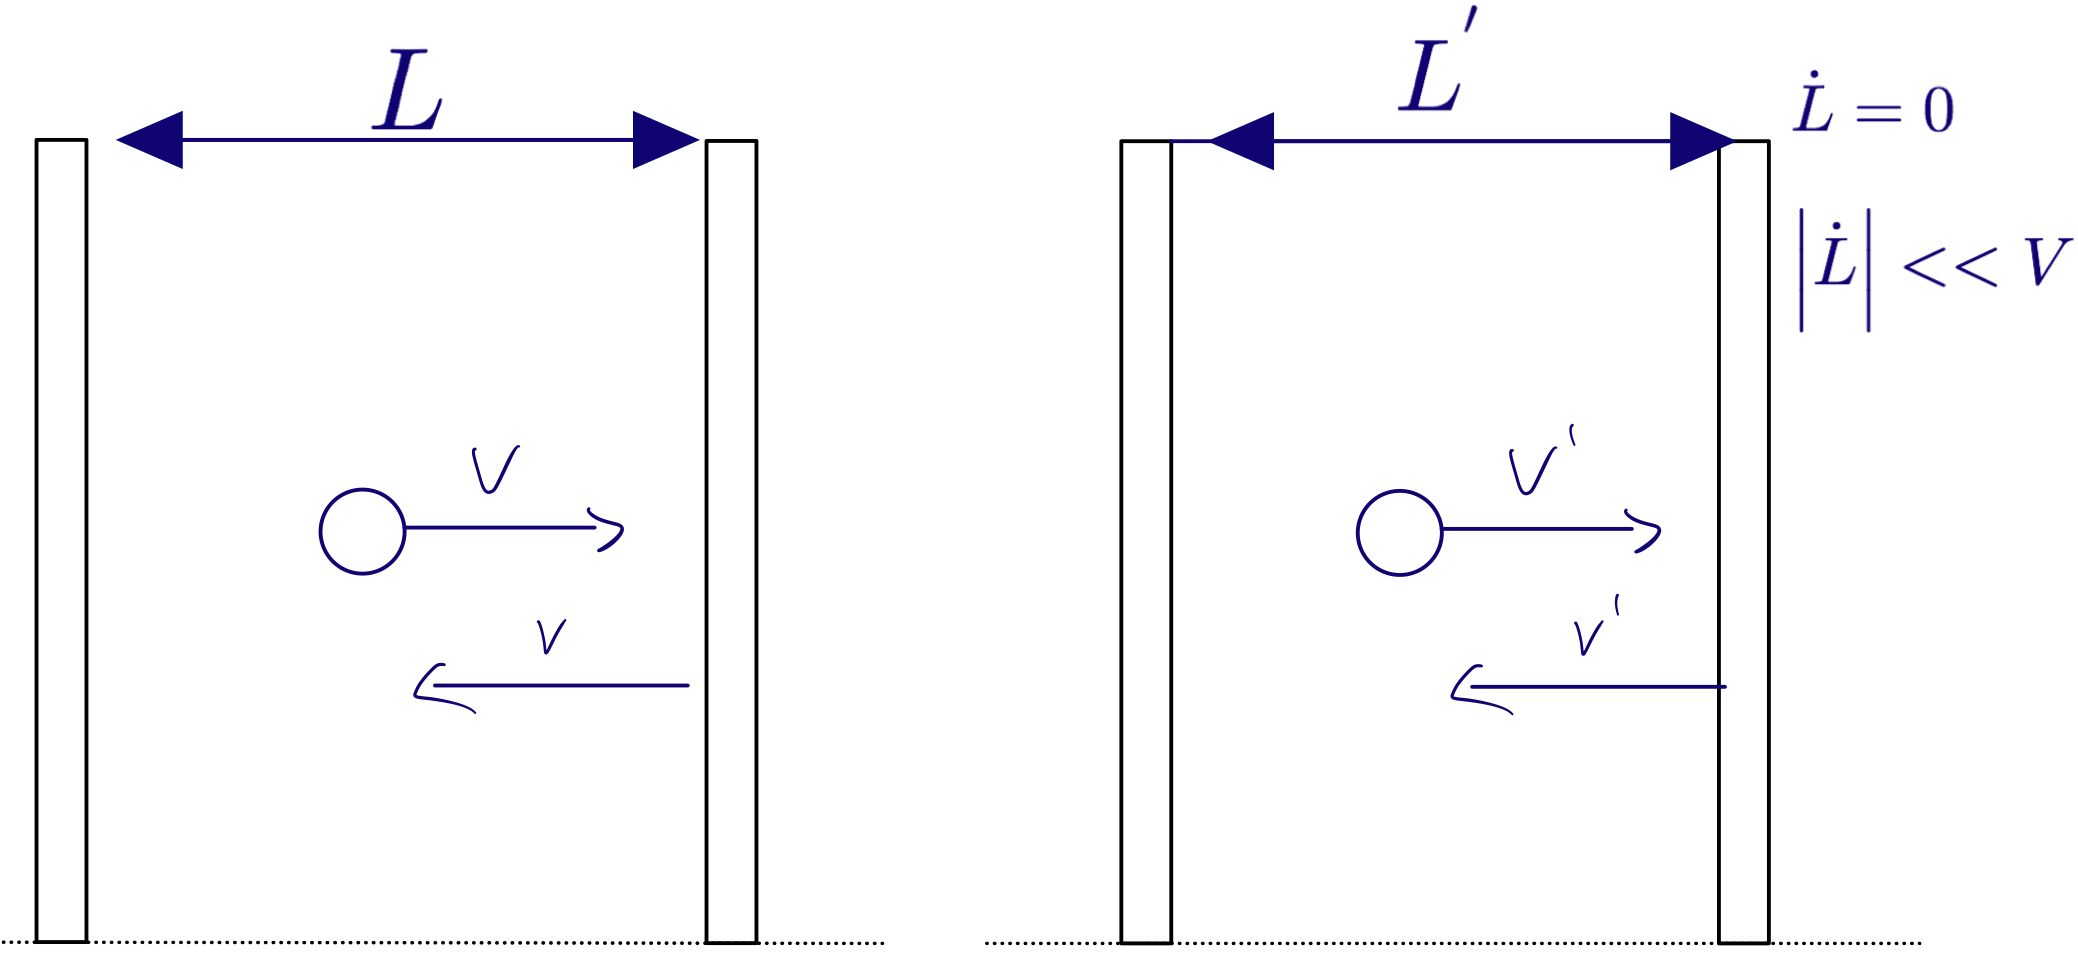
\includegraphics[width=0.5\textwidth]{diagrama_pelota.png}
    \caption{Diagrama de pelota rebotando}
    \label{d_pe}
\end{figure}
Con esto, se dibuja el espacio de fases de la pelota teniendo:

\begin{figure}[h!]
    \centering
    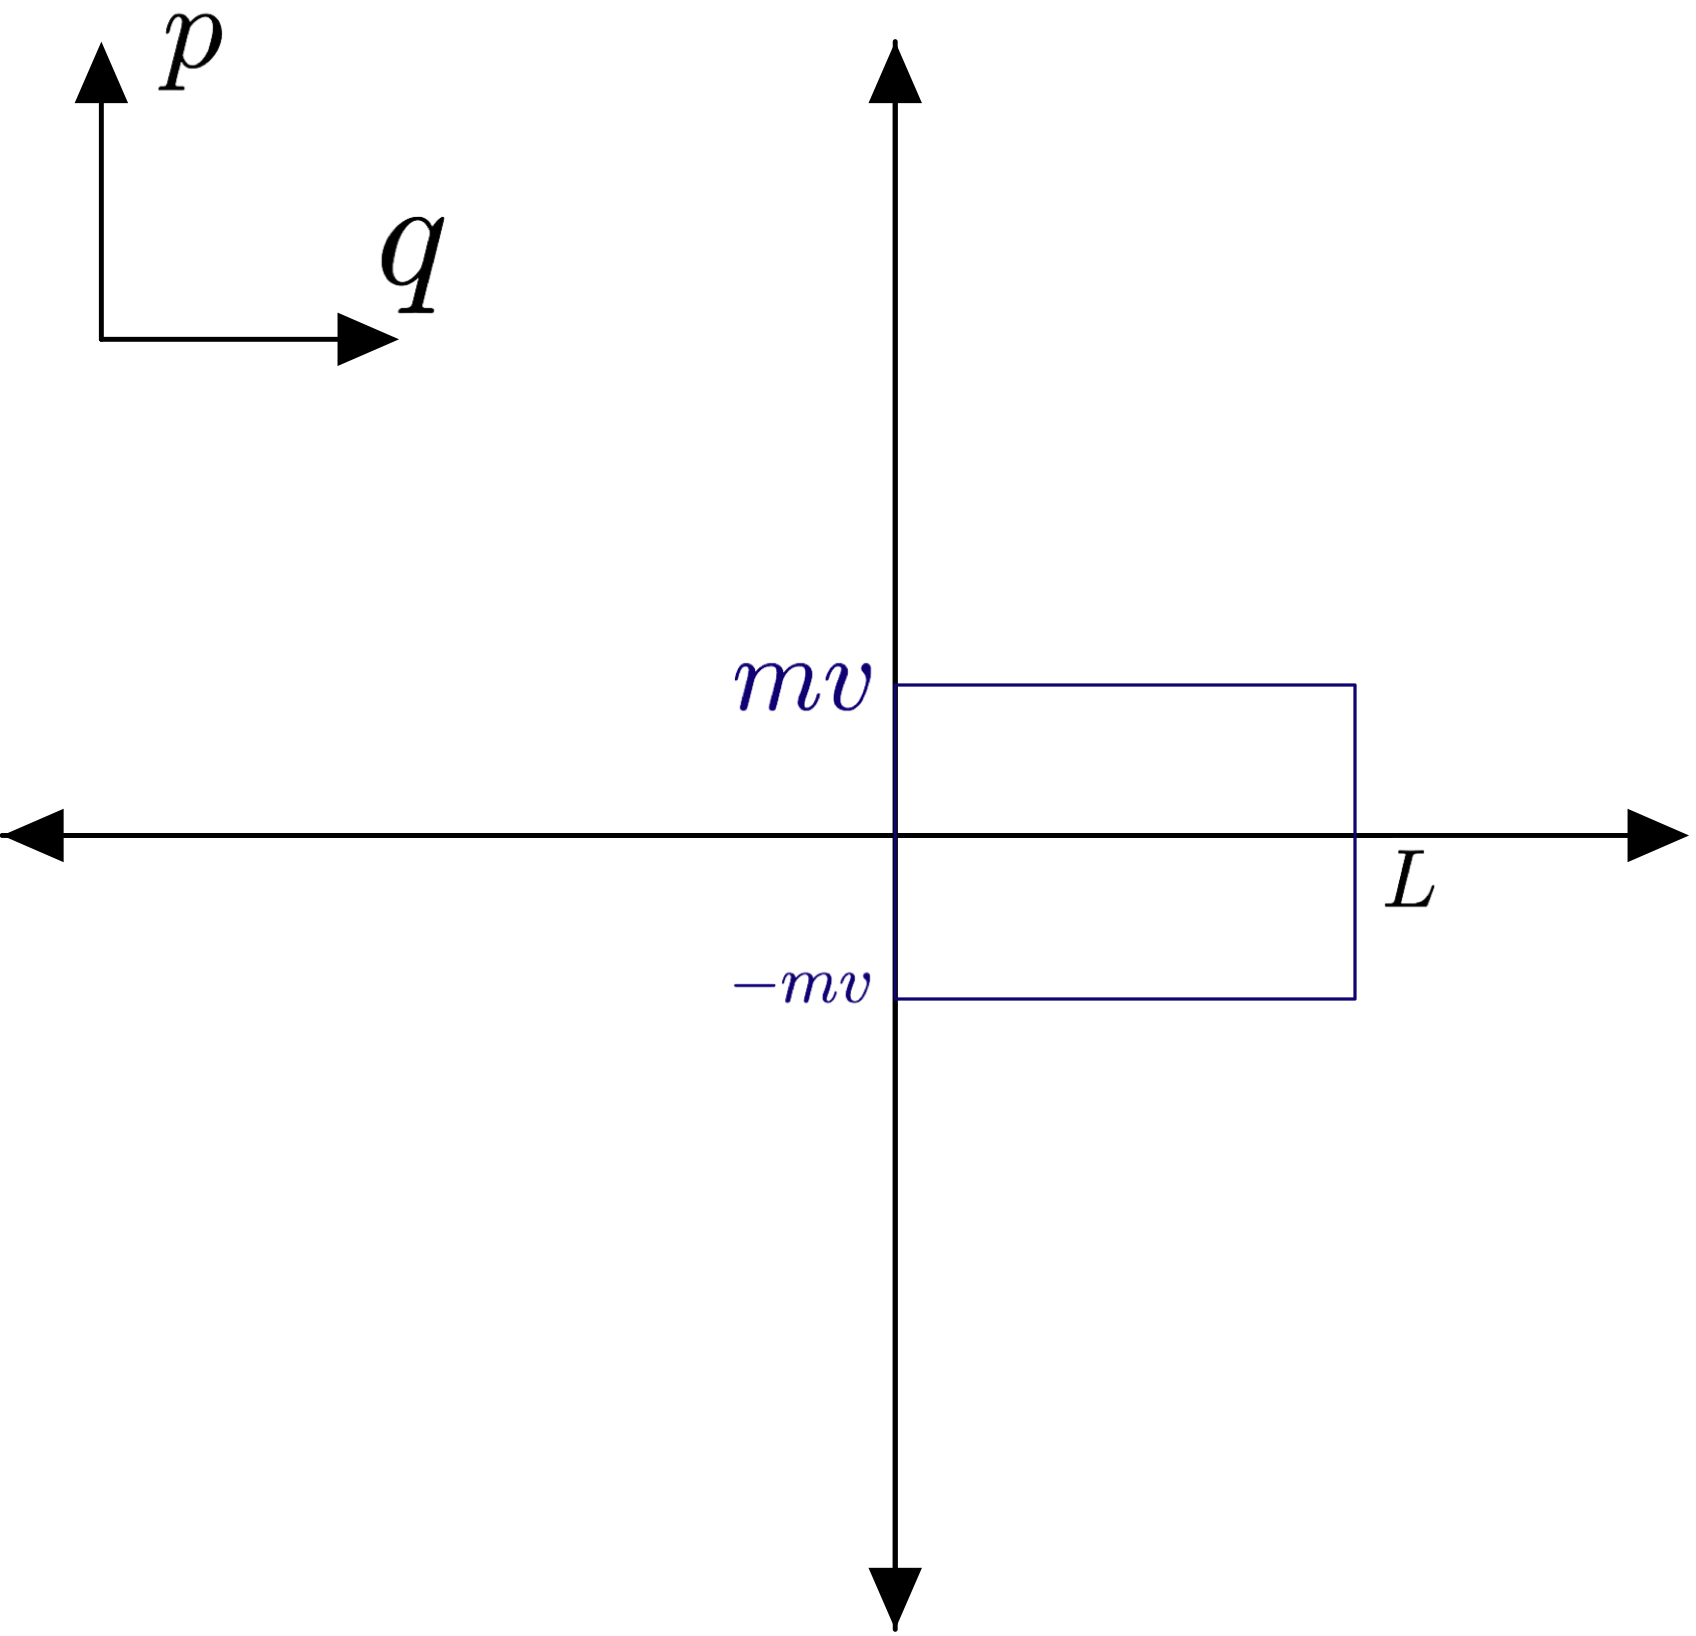
\includegraphics[width=0.5\textwidth]{ef_pe.png}
    \caption{Espacio de fases pelota rebotando}
    \label{ef_pe}
\end{figure}
Con esto es sencillo calcular J,
\begin{align}
J=\inv{2\pi} Area\\
J= \inv{2\pi} L 2mv\\
J= \inv{\pi}mvL	
\end{align}
Si el cambio es adiabatico, la velocidad crecera como $\inv{L}$.\\
Esta ecuacion permite modelar la ecuacion de estado de un gas ideal monoatomico metido en una caja usando pavo-raton. \\
\item Pendulo de longitud variable con pequeñas oscilaciones\\
	\begin{align}
	J=\frac{E}{\omega}=\inv{2}ml^2 \omega^2 \theta^2\\
	J=ml^2 \sqrt{g}{l}\theta^2	\\
	J= m\sqrt{g} \qty(l^{\frac{3}{4}}\theta)^2\\
	\theta_{max}=\inv{l^{\frac{3}{4}}}\\
	\end{align}
	\item Particula cargada en un campo magnetico uniforme que cambia suavemente\\
	$$\vec{B}=B \hat{z}$$
\begin{figure}[h!]
    \centering
    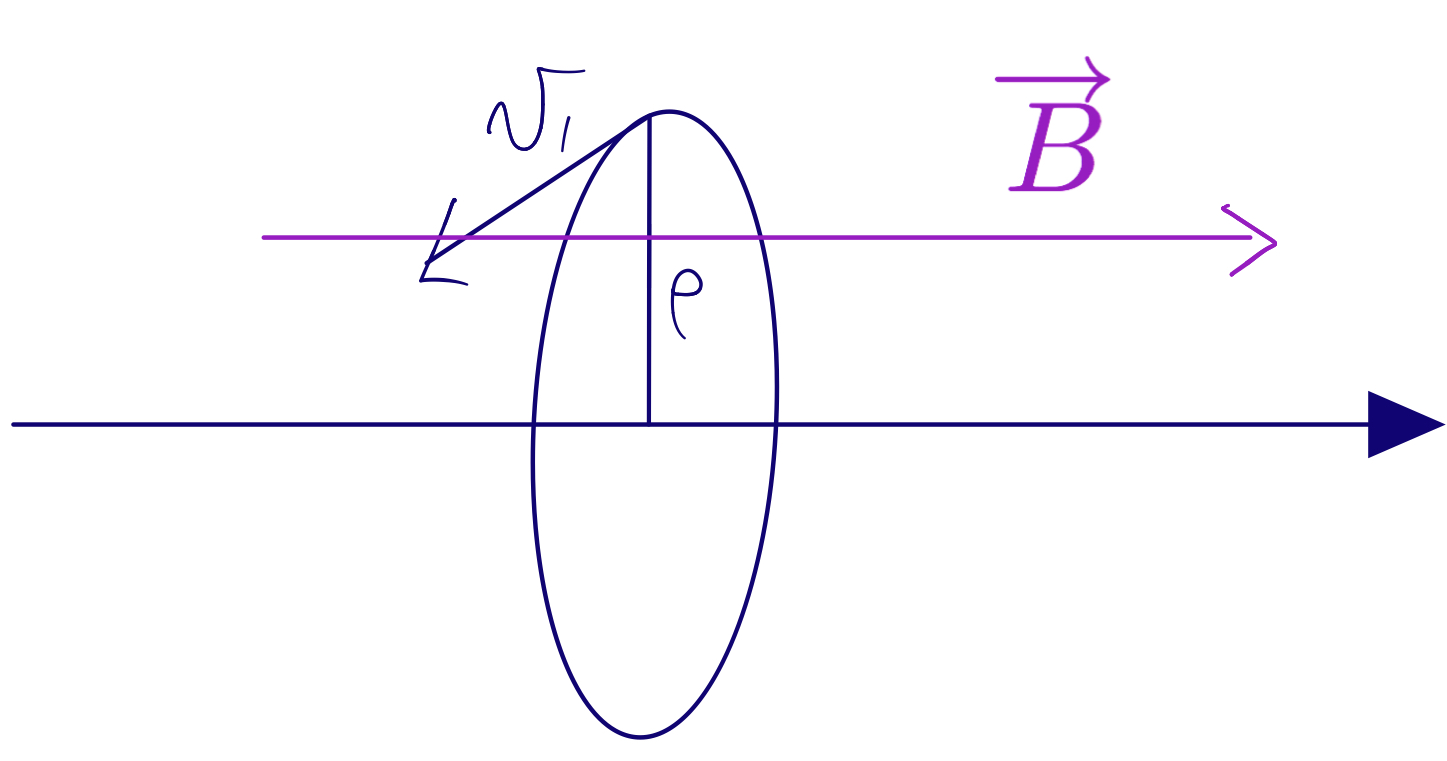
\includegraphics[width=0.5\textwidth]{dg_cm.png}
    \caption{Diagrama de campo magnetico uniforme}
    \label{dg_cm}
\end{figure}	
\begin{align}
v_\perp	=\frac{qB\rho}{mc}\\
J=\inv{2\pi}\oint p\,  dq\\
\vec{p}=\qty(m\vec{v} + \frac{\rho}{c}\vec{A})\\
J = inv{2\pi} \oint \qty(m\vec{v} + \frac{\rho}{\rho}\vec{A}) \, d\vec{l}\\
J= - \rho \frac{B\rho^2}{c} \rightarrow Flujo
\end{align}
Como la energía es constante, si esta se mueve por el cambio que varia y se va acercando cada vez mas hacia la parte con mayor densidad. Generado una botella magnético\footnote{Se trata de usar eso en fusion nuclear.
Se ve esto en los cinturones de Van Hallen. En 1911 Lorentz y Einstein se pusieron a discutir sobre el cambio del largo de un pendulo cuántico mediante el mismo principio usado anteriormente y surgió que quizás habría que cuantificar las variables clásicas que no cambian sobre cambios lentos.\\ Esto fue conocido como la regla de cuantificación de Bohr-Sommerfield.}.\\
\end{enumerate}
\s{Ecuación de Hamilton-Jacobi}
Esta es solo 1 ecuación con n grados de libertad, pero una sola.\\
Es una ecuacion complicada en derivadas parciales para una función generatriz $F_2(q,p,t)$. Con un único objetivo, que nos de un Hamiltoniano mas simple posible.
\begin{align}
 \H(q,p,t) \xrightarrow{T.C} \H'(Q,P)=0	
\end{align}

El objetivo es que las nuevas Q y P serán constantes determinadas por sus condiciones iniciales.\\
\begin{align}
\H'= \H + \pdv{F_2}{t}\bigg/\textit{Notacion: }F_2(Q,P,t) = S(Q,P,t)\\
	p_i = \pdv{F}{q_i}\\
\rojo{\boxed{\H(\xn{q},\xn{\pdv{S}{q}},t) +\pdv{S}{t}=0}}
\end{align}
La Funcion que resuelve la Ecuacion de Hamilton-Jacobi se llama Funcion principal de Hamilton $(S)$.
\newpage
\ej
\eq{\textit{Oscilador Armonico}}
\begin{align}
\H = \pdv{p^2}{2m} + \frac{m\omega^2}{2}q^2
\end{align}
Cómo se lee la ecuación de Hamilton-Jacobi?\\
Donde diga p en el $\H$ reemplazamos por $\pdv{S}{q}$. \\
\begin{align}
\inv{2m}\qty(\pdv{S}{q})^2 + 	\frac{m\omega^2}{2}q^2 + \azulf{\pdv{S}{t}=0}
\end{align}
La dependencia entre q,t es separable. Con un ansatz veremos $S=W(Q)+T(t)$ es una prueba para ver si es separable.
\begin{align}
&\inv{2m} \qty(\dv{W}{q})^2 + \inv{2} m\omega^2 q^2 +\dv{T}{t}=0\\
&\inv{2m} \qty(\dv{W}{q})^2 + \inv{2} m\omega^2 q^2 =-\dv{T}{t}= E\\
&\therefore -\dv{T}{t}= E \implies T(t)=-Et\\
&\inv{2m} \qty(\dv{W}{q})^2 + \inv{2} m\omega^2 q^2=E\\
&\dv{W}{q}= \sqrt{2m\qty(E-m\omega^2 q^2)}\\
&W(q)=\intt{0}{q} \sqrt{2m\qty(E-m\omega^2 q'^2)}\, dq'\\
&S= W(q)-Et\\
&p=\pdv{S}{q}=\dv{W}{q}\vl Q=\pdv{S}{P} \vl \textit{Constante de IntegracionÑ }P=E\\
&Q=\pdv{S}{P}=\pdv{S}{E}- \pdv{W}{E}-t=\beta\\
&W(q)= \inv{\omega} \arcsin{\sqrt{\frac{m \omega^2}{2E}}q} = \omega t +\omega \beta\\
&q= \sqrt{\frac{2E}{m \omega^2}} \sinn{\omega t +\phi}
\end{align}
Esto nos muestra que esta ecuacion nos lleva del Hamiltoniano y nos retrotrae a las condiciones iniciales.Esto se parece mucho a la Ecuacion de Schrodinger.\\
Esto que vimos de trabajar en variables separables ocurre siempre que el Hamiltoniano sea constante.
\ss{Separacion de variables en la Ecuacion de Hamilton-Jacobi}
\begin{align}
\H(\xn{q},\xn{p}), independiente\\
\boxed{S= W(\xn{q},\xn{\alpha})-Et}\label{op2}
\end{align}
Cuando la \eqreff{op2} ocurre se llama \textbf{Funcion caracteristica de Hamilton}. Particularmente son interesantes cuando la funcion caracteristica tambien sea separable o parcialmente. \\
\begin{enumerate}
\item Es totalmente separable si
\en{W=\sumn{i} W_i (\xn{q},\xn{\alpha})}
\end{enumerate}
Un caso interesante es cuando una de las coordenadas q es cíclica. Si es cíclica, se puede demostrar que esa coordenada se va a separar y se puede escoger como constante a ese valor integrado se escogerá como constante de condición inicial.
\eq{Mov.Periodico \rightarrow Conviene \,\,\,\,\, \theta,J}
\eq{P_i=J_i = \inv{2\pi}\oint p_i \,dq_i = \inv{2\pi} \oint \dv{W_i}{q_i}  \, dq_i}
\begin{align}
Q_i = \pdv{S}{J_i}=\dv{W_i}{J_i}- \pdv{\H}{J_i}t=\theta_i - W_i t\implies \theta_i = W_i + \beta_i
\end{align}
Es interesante si elegimos como nuevo momento las variables de acción, se obtienen las condiciones de las variables de ángulo. \\
\ej
\eq{\textit{Problema de Keppler}}
\begin{align}
\H= \frac{p_r^2}{2m}+ \frac{p_\theta^2}{2mr^2}-\frac{k}{r},\,\, k = Gm_1m_2\\
HJ= \inv{2m} \qty[\qty(\pdv{S}{r})^2 + \frac{r^2}\qty(\pdv{S}{\theta})^2] - \frac{k}{r}+\pdv{S}{t}	=0
\end{align}
Ansatz; $S= W_r(r)+ W_\theta (\theta) -Et$\\
\begin{align}
	\inv{2m} \qty[\qty(\pdv{W_r}{r})^2 + \frac{r^2}\qty(\pdv{W_\theta}{\theta})^2] -Et	=0\\
\frac{r^2}{2m} 	\qty(\pdv{W_r}{r})^2 - kr- Er^2=-\inv{2m}\qty(\pdv{W_\theta}{\theta})^2=-\frac{l^2}{2m}\\
\dv{W}{\theta}=l \implies W_\theta = l \, \theta\\
\inv{2m}\qty(\dv{W_r}{r})^2 - \frac{k}{r}-E+\frac{l^2}{2mr^2}=0\\
W_r = \intt{0}{r}\sqrt{2m\qty(E+\frac{k}{r})-\frac{l^2}{r^2}}\,dr
\end{align}
Trayectorias
\begin{align}
Q_\theta=\beta_\theta=\pdv{S}{l}=\theta +\pdv{W}{l}=cte\\
\theta= \beta_\theta - \pdv{W}{l}\rightarrow \theta(r) \,;\,r(\theta)
\end{align}
Dependencia temporal:
\begin{align}
Q_r=\beta_E = cte\\
Q_r=\pdv{S}{E}= -t+\pdv{W_r}{E}\\
t= \beta_E - \pdv{W_e}{E}\rightarrow t=t(r)\,:\, r(t)
\end{align}
Enfatizar que las ventajas de tener variables de accion en problemas periodicos.
\eq{\textbf{Variables de accion}}
\begin{align}
J_\theta = \inv{2\pi} \oint p_\theta \, d\theta =l\\
J_r= 	 \inv{2\pi} \oint p_r = \inv{2\pi} \oint \pdv{S}{r} \, dr = \inv{2\pi} 2\intt{r-}{r+} \dv{W_r}{r}\, dr\\
J_r =  k \sqrt{\frac{m}{2|E|}}-l
\end{align}




\end{document}